\documentclass{article}

\newcommand{\myname}{Tan Yee Jian (A0190190L)}
\newcommand{\mytitle}{CS2309 Homework 1}
\title{\mytitle}
\author{\myname}
\date{\today}

\usepackage[a4paper]{geometry}
\usepackage[utf8]{inputenc}
\usepackage[T1]{fontenc}
\usepackage{textcomp}
\usepackage{amsmath, amssymb, amsthm}
\theoremstyle{plain}
\usepackage{hyperref}
% \usepackage[outputdir=tmp]{minted}
% \usepackage{lmodern}
\usepackage{tgpagella}
\usepackage{fancyhdr}
\usepackage{lastpage}
\pagestyle{fancy}
\fancyhf{}
% \rhead{Page \thepage/\pageref{LastPage}}
\rhead{Page \thepage}
\lhead{\myname}
\chead{\mytitle}
\usepackage{graphicx}

% \usepackage{tocloft}
% \usepackage[thinc]{esdiff}
% \renewcommand{\thesection}{Question \arabic{section}}
% \renewcommand{\thesubsection}{Part \arabic{section}(\roman{subsection})}
% \renewcommand{\thesubsubsection}{Solution}
% \cftsetindents{subsection}{1.5em}{4.5em}
% \cftsetindents{subsubsection}{3.8em}{5.5em}

\newcommand{\pmat}[1]{ \begin{pmatrix}#1\end{pmatrix} }
\newcommand{\seqn}[1]{(#1)^\infty_{n=1}}
\newcommand{\seqk}[1]{(#1)^\infty_{k=1}}
% (series term): returns a series with counter n=1 to \infty.
\newcommand{\infsrsn}[1]{\sum\limits^\infty_{n=1}#1}
\newcommand{\infsrsk}[1]{\sum\limits^\infty_{k=1}#1}
\newcommand{\R}{\mathbb{R}}
\newcommand{\N}{\mathbb{N}}
\newcommand{\Q}{\mathbb{Q}}
\newcommand{\Z}{\mathbb{Z}}
\newcommand{\C}{\mathbb{C}}
\newcommand{\F}{\mathbb{F}}
\newcommand{\cmm}{C(M_1,M_2)}
\newcommand{\met}[1]{\langle M_{#1},\rho_{#1}\rangle}
\newcommand{\ntoinf}{\limits_{n\to\infty}}
\newcommand{\ktoinf}{\limits_{k\to\infty}}
% \newcommand{\onetoinf}[]{^\infty_{n=1}}
\newcommand{\limn}[1]{\lim\ntoinf #1}
\newcommand{\limk}[1]{\lim\ktoinf #1}

\DeclareMathOperator{\spn}{span}
\DeclareMathOperator{\diam}{diam}

\begin{document}
\maketitle
% \tableofcontents
\section{Expectation}
I hope this module can force me to read some research papers and formulate my
own research idea for my Final Year Project next year, which I hope to be a
interdisciplinary paper between Pure Mathematics and Computer Science, for
example in the area of Type Theory and Constructive Mathematics. I also hope to
survey other fields in theoretical CS and find something that I might be
interested in.

\section{Research Interest}
My research interest is currently related to Type Systems, Theorem Proving and
possibly Software Verification. I am interested about how type system can not
only bring about safer programs, furthermore verify programs in terms of
mathematical proofs, which guarantees correctness. Theoretically, I am
interested in the modelling of computation in Type Theory (lambda calculus),
Proof Theory (mathematical logic) and possibly Category Theory as well.

\begin{figure}[h]
\centering
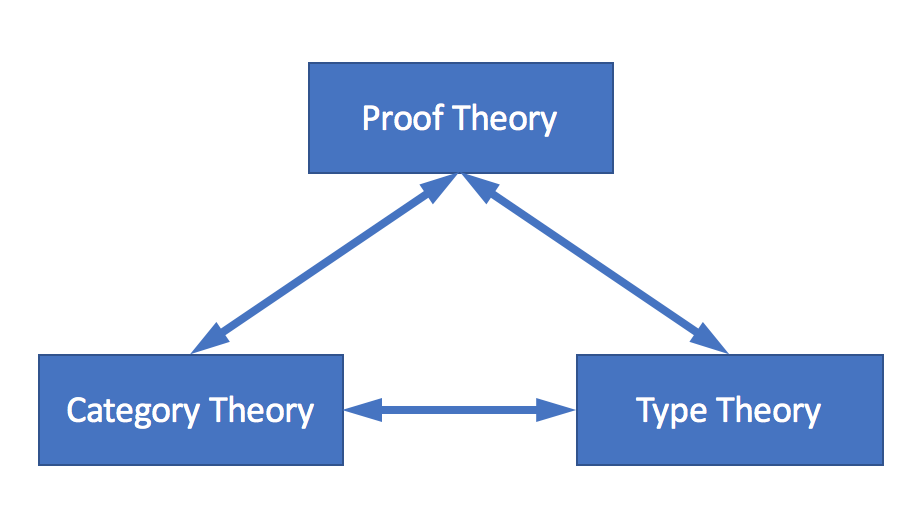
\includegraphics[width=0.8\textwidth]{type-proof-cat.png}
\caption{The 3-way correspondence between Proof, Type and Category Theories.}
\end{figure}

\section{General awareness}

\href{https://corporate.shopback.com/}{Shopback} is a wildly successful
Singapore startup, one of whose product I use on a daily basis. Started in 2014,
it has now offices in 9 countries and counting. Same as all internet and
shopping companies, it has a tech team which is at the forefront of innovation
(see \href{https://medium.com/shopback-tech-blog}{Technical Blog}), especially
when they now extend their services from providing cashback to shopping, which
immediately brings about the issues in
\href{https://medium.com/shopback-tech-blog/build-ranking-in-a-real-world-search-application-random-thoughts-7d98df0996aa}{Search
  Ranking} and
\href{https://medium.com/shopback-tech-blog/part-1-merchants-recommendation-with-gru4rec-and-offline-evaluation-3235e6242d79}{Merchant
  Evaluation}, and the challenges and their solutions are documented well on the
technical blog.

\end{document}
